\documentclass[compress]{beamer}
\usepackage{ifthen,verbatim}

\newcommand{\isnote}{}
\xdefinecolor{lightyellow}{rgb}{1.,1.,0.25}
\xdefinecolor{darkblue}{rgb}{0.1,0.1,0.7}

%% Uncomment this to get annotations
%% \def\notes{\addtocounter{page}{-1}
%%            \renewcommand{\isnote}{*}
%% 	   \beamertemplateshadingbackground{lightyellow}{white}
%%            \begin{frame}
%%            \frametitle{Notes for the previous page (page \insertpagenumber)}
%%            \itemize}
%% \def\endnotes{\enditemize
%% 	      \end{frame}
%%               \beamertemplateshadingbackground{white}{white}
%%               \renewcommand{\isnote}{}}

%% Uncomment this to not get annotations
\def\notes{\comment}
\def\endnotes{\endcomment}

\setbeamertemplate{navigation symbols}{}
\setbeamertemplate{headline}{\mbox{ } \hfill
\begin{minipage}{5.5 cm}
\vspace{-0.75 cm} \small
\end{minipage} \hfill
\begin{minipage}{4.5 cm}
\vspace{-0.75 cm} \small
\begin{flushright}
\ifthenelse{\equal{\insertpagenumber}{1}}{}{Jim Pivarski \hspace{0.2 cm} \insertpagenumber\isnote/\pageref{numpages}}
\end{flushright}
\end{minipage}\mbox{\hspace{0.2 cm}}\includegraphics[height=1 cm]{../cmslogo} \hspace{0.1 cm} \includegraphics[height=1 cm]{../tamulogo} \hspace{0.01 cm} \vspace{-1.05 cm}}

\begin{document}
\begin{frame}
\vfill
\begin{center}
\textcolor{darkblue}{\Large Muon Alignment with CRAFT-2009 Data}

\vfill
\begin{columns}
\column{0.3\linewidth}
\begin{center}
\large
\textcolor{darkblue}{Jim Pivarski}
\end{center}
\end{columns}

\begin{columns}
\column{0.3\linewidth}
\begin{center}
\scriptsize
{\it Texas A\&M University}
\end{center}
\end{columns}

\vfill
 8 September, 2009

\end{center}
\end{frame}

%% \begin{notes}
%% \item This is the annotated version of my talk.
%% \item If you want the version that I am presenting, download the one
%% labeled ``slides'' on Indico (or just ignore these yellow pages).
%% \item The annotated version is provided for extra detail and a written
%% record of comments that I intend to make orally.
%% \item Yellow notes refer to the content on the {\it previous} page.
%% \item All other slides are identical for the two versions.
%% \end{notes}

\small

\begin{frame}
\frametitle{Outline}
\begin{itemize}\setlength{\itemsep}{0.75 cm}
\item Reminder of the methods
\item Status of hardware alignment reconstruction
\item Preliminary DT results from tracks
\item Preliminary CSC results from tracks
\end{itemize}
%% \hspace{-0.83 cm} \textcolor{darkblue}{\Large Outline2}
\end{frame}

\begin{frame}
\frametitle{Reminder of the methods}
\framesubtitle{(with a new name)}

\hfill \includegraphics[width=3.5 cm]{reference-target.png}

\vspace{-2.3 cm}
\begin{itemize}\setlength{\itemsep}{0.5 cm}
\item \textcolor{darkblue}{Reference-Target (R-T):} align a Target set \\ of chambers using globalMuon tracks
  from \\ a fixed Reference (tracker)

{\it (The Algorithm Formerly Known as \textcolor{darkblue}{``HIP''})}

{\scriptsize Came up in paper-draft process: spirit of the procedure is different from HIP \\ Also, software module is named MuonAlignmentFromReference, not HIP}

\item \textcolor{darkblue}{Millepede (future):} combine local segment
  and globalMuon data into one fit.  \textcolor{darkblue}{(Now):} reproduce R-T with globalMuons only

\vspace{-0.1 cm}
\hfill \includegraphics[width=1.5 cm]{overlaps.png}

\vspace{-2.1 cm}
\item \textcolor{darkblue}{CSC-Overlaps:} reconstruct CSC ring
  geometry using \\ local segments that overlap along the CSC edges

\item \textcolor{darkblue}{Barrel, endcap, and link hardware systems:}
  reconstruct geometry from external measurements
\end{itemize}
\end{frame}

\begin{frame}
\frametitle{Status of hardware reco}

\begin{itemize}\setlength{\itemsep}{0.25 cm}
\item All systems read out for most of CRAFT-2009
\begin{itemize}
\item endcap read out until Aug~25 (LV problem)
\end{itemize}
\item Preliminary geometries built from barrel and link data, studies
  of stability and dependence on $\vec{B}$
\begin{itemize}
\item soon will be in a form that can be compared with track-based
  results
\end{itemize}
\end{itemize}

\vfill
{\large CRAFT-2009 barrel response to $\vec{B}$:}
\begin{center}
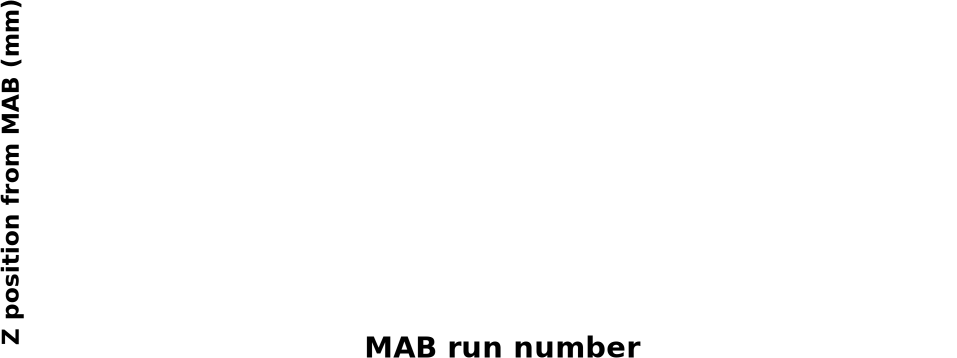
\includegraphics[width=0.75\linewidth]{hardware_reco.pdf}
\end{center}

\vspace{-0.5 cm}
\hfill \textcolor{darkblue}{\scriptsize B\'eni No\'emi, Szill\'asi Zolt\'an}
\end{frame}

\begin{frame}
\frametitle{Prelim.\ track-based DT results}

\begin{itemize}
\item Track-based procedures tuned in CRAFT-2008
\begin{itemize}
\item identified and responded to the most important propagation
  effects in real data {\scriptsize ($\vec{B}(\vec{x})$, non-Gaussian tails, $x$-$\frac{dx}{dz}$ correlation)}
\end{itemize}
\item Applied exactly the same procedure in 2009 {\scriptsize (now an automated script)}
\begin{itemize}
\item below: differences in each degree of freedom, for each chamber
\item grey: unaligned 2008 $\to$ aligned 2008 {\scriptsize (broad, systematic)}
\item yellow: aligned 2008 $\to$ aligned 2009 {\scriptsize (narrower, especially angles)}
\end{itemize}
\end{itemize}

\begin{columns}
\column{0.16\linewidth}
\begin{center}
translational degrees of freedom

\vspace{0.75 cm}
rotational degrees of freedom

\vspace{0.5 cm}
\mbox{ }
\end{center}
\column{0.8\linewidth}
\includegraphics[height=\linewidth, angle=90]{v4_2008_2009.pdf}
\end{columns}
\end{frame}

\begin{frame}
\frametitle{DT translations by wheel}

\begin{columns}
\column{0.65\linewidth}
\includegraphics[width=\linewidth]{phipos_yprime_2008_2009.pdf}
\column{0.35\linewidth}
\begin{itemize}
\item Collective motion correlated by wheel

\mbox{\hspace{-1.2 cm}
\begin{minipage}{5 cm}
\begin{tabular}{l c c}
& \scriptsize $\phi$ (mrad) & \scriptsize $z$ (mm) \\
\scriptsize wheel $-$1 & \scriptsize $-0.28$ & \scriptsize $0.34$ \\
\scriptsize wheel    0 & \scriptsize $-0.02$ & \scriptsize $-0.16^*$ \\
\scriptsize wheel $+$1 & \scriptsize $-0.39$ & \scriptsize $-1.74$
\end{tabular}
\end{minipage}}

{\scriptsize $^*$not including outliers}

\item Only wheel~0 stationary relative to tracker

\item 4 out of 8 outliers identified as chambers that were moved between
  CRAFTs \textcolor{red}{(red)}

\hfill \textcolor{darkblue}{\scriptsize Alberto Benvenuti}
\end{itemize}

\end{columns}
\end{frame}

\begin{frame}
\frametitle{DTs vs.~time}

\begin{columns}
\column{0.6\linewidth}
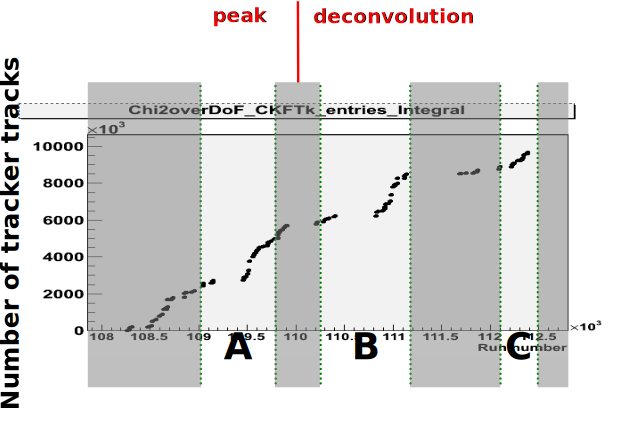
\includegraphics[width=\linewidth]{bfield_regions.pdf}
\column{0.4\linewidth}
\begin{itemize}
\item Three $B=3.8$~T periods in CRAFT-2009
\item Align each independently, observe differences
\item Below: \only<1>{$r\phi$ positions}\only<2>{$z$ positions}

\only<2>{(moved chambers \textcolor{red}{red})}
\end{itemize}
\end{columns}

\vfill
\only<1>{\includegraphics[height=\linewidth, angle=90]{vstime_bfield.pdf}}
\only<2>{\includegraphics[height=\linewidth, angle=90]{vstime_bfield_y.pdf}}
%% vstime_bfield_norm.pdf
\end{frame}

\begin{frame}
\frametitle{Prelim.\ track-based CSC results}

\begin{itemize}
\item Largest misalignments are in the disk positions
\item Standard diagnostic plot (used to understand DTs in 2008):
  residuals versus $\phi$ from $-\pi$ to $\pi$, with smaller binning
  \mbox{than chambers\hspace{-1 cm}}

  {\scriptsize \textcolor{darkblue}{Shades of} \textcolor{blue}{blue} are 2-D histogram, black points are profile, \textcolor{red}{red curve} is disk-fit}

\item Complete $\phi$ coverage makes disk fit \mbox{\scriptsize ($\delta_{\phi_z}+\delta_x\sin\phi+\delta_y\cos\phi$)} robust
\end{itemize}

\begin{columns}
\column{0.75\linewidth}
\includegraphics[height=\linewidth, angle=90]{demonstrate_2008.pdf}

\includegraphics[height=\linewidth, angle=90]{demonstrate_2009.pdf}
\column{0.2\linewidth}
\begin{center}
ME$+$1/1

CRAFT-2008

CMSSW\_2\_2\_11

\vspace{1.5 cm}
ME$+$1/1

CRAFT-2009

CMSSW\_3\_1\_2

\vspace{0.5 cm}
\mbox{ }
\end{center}
\end{columns}
\end{frame}

\begin{frame}
\frametitle{Prelim.\ track-based CSC results}

\vspace{-0.3 cm}
\begin{columns}
\column{0.7\linewidth}
\begin{itemize}
\item Chamber angles are (nearly) independent of disk position
\item Can clearly observe individually rotated chambers from ``angle residuals''
\end{itemize}

\column{0.3\linewidth}
\vspace{0.7 cm}
\includegraphics[width=\linewidth]{explanation.pdf}
\end{columns}

\vfill
\begin{columns}
\column{0.75\linewidth}
\includegraphics[height=\linewidth, angle=90]{correspondance_2008_mep32_phiy.pdf}

\includegraphics[height=\linewidth, angle=90]{correspondance_2009_mep32_phiy.pdf}
\column{0.2\linewidth}
\begin{center}
ME$+$3/2

CRAFT-2008

CMSSW\_2\_2\_11

\vspace{1.5 cm}
ME$+$3/2

CRAFT-2009

CMSSW\_3\_1\_2

\vspace{0.5 cm}
\mbox{ }
\end{center}
\end{columns}
\end{frame}

\begin{frame}
\frametitle{Correspondance with beam-halo}

\vspace{0.5 cm}
\begin{columns}
\column{0.3\linewidth}
\includegraphics[width=\linewidth]{csc_alignments.png}

\column{0.3\linewidth}
\scriptsize
Correlation between globalMuon (cosmics) and \textcolor{red}{local segments (beam-halo)}

\vspace{0.2 cm}
Some statistically significant changes \\ 2008 $\to$ 2009

\vspace{0.2 cm}
$\phi_y$: the only parameter that couldn't be validated with \mbox{photogrammetry (PG)\hspace{-1 cm}}

\column{0.3\linewidth}
\includegraphics[width=\linewidth]{csc_coordinates.pdf}
\end{columns}

\vspace{0.5 cm}
\includegraphics[height=\linewidth, angle=90]{beamhalo_2009_mem21.pdf}
\end{frame}

\begin{frame}
\frametitle{Problem to be solved\ldots}

\begin{itemize}
\item ME$x$/2 rings have disk displacement plus even-odd \mbox{chamber alternation\hspace{-1 cm}}
\item New in 2009 or 31X, not a likely physical motion
\begin{itemize}
\item stands in the way of performing an endcap alignment
\end{itemize}
\item It's bracketed between releases; currently ruling out culprits\ldots
\end{itemize}

\begin{columns}
\column{0.75\linewidth}
\includegraphics[height=\linewidth, angle=90]{alternation_2008_mem12_design.pdf}

\includegraphics[height=\linewidth, angle=90]{alternation_2009_mem12_design.pdf}
\column{0.2\linewidth}
\begin{center}
ME$-$1/2

CRAFT-2008

CMSSW\_2\_2\_11

\vspace{1.5 cm}
ME$-$1/2

CRAFT-2009

CMSSW\_3\_1\_2

\vspace{0.5 cm}
\mbox{ }
\end{center}
\end{columns}
\end{frame}

\begin{frame}
\frametitle{Conclusions}
\begin{itemize}\setlength{\itemsep}{0.2 cm}
\item Hardware alignment getting to the point where comparisons with track-based alignment will be possible
\item Reference-Target (HIP) algorithm is stable, can now be used to
  trace time-dependencies in DT alignment
\item Cosmic track reconstruction in endcap significantly improved \mbox{($\phi$ coverage)},
  making disk alignment more robust
\item Comparison of globalMuon method and local segment method is a
  stringent cross-check with different systematics
\begin{itemize}
\item ideally suited to $pp \to \mu X$, where we can apply both methods at the same time (with the same tracks or exclusive sets)
\end{itemize}
\item Constants readiness:
\begin{itemize}
\item DTs: some tweaks, but essentially ready
\item CSCs: need to find and fix a (likely) bug
\end{itemize}
\end{itemize}
\label{numpages}
\end{frame}

% \section*{First section}
\begin{frame}
\begin{center}
\Huge \textcolor{blue}{Backup}
\end{center}
\end{frame}

\begin{frame}
\frametitle{DTs vs.~time}

\begin{columns}
\column{0.6\linewidth}
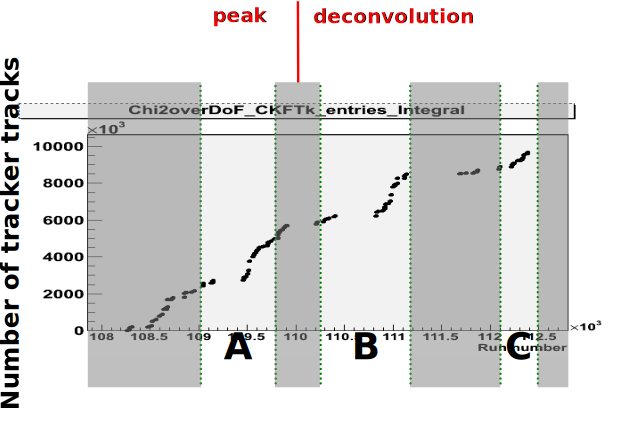
\includegraphics[width=\linewidth]{bfield_regions.pdf}
\column{0.4\linewidth}
\begin{itemize}
\item Three $B=3.8$~T periods in CRAFT-2009
\item Align each independently, observe differences
\item Below: normalized $r\phi$ positions
\end{itemize}
\end{columns}

\vfill
\only<1>{\includegraphics[height=\linewidth, angle=90]{vstime_bfield_norm.pdf}}
\end{frame}

\begin{frame}
\frametitle{Prelim.\ track-based CSC results}

\renewcommand{\arraystretch}{1.2}
\begin{tabular}{c c c c c}
\scriptsize Station & \scriptsize Rotation (mrad) & \scriptsize $x$ translation (mm) & \scriptsize $y$ translation (mm) & \scriptsize $\chi^2/N_{\mbox{dof}}$ \\
\scriptsize ME$+$3 & \scriptsize $-0.2$ $\pm$ $ 0.1$ & \scriptsize $ 4.3$ $\pm$ $ 0.2$ & \scriptsize $-2.1$ $\pm$ $ 0.3$ & \scriptsize 3.6663 \\
\scriptsize ME$+$2 & \scriptsize $-0.5$ $\pm$ $ 0.1$ & \scriptsize $ 4.3$ $\pm$ $ 0.2$ & \scriptsize $-2.0$ $\pm$ $ 0.2$ & \scriptsize 2.2600 \\
\scriptsize ME$+$1 & \scriptsize $-0.11$ $\pm$ $ 0.04$ & \scriptsize $ 4.7$ $\pm$ $ 0.1$ & \scriptsize $ 1.2$ $\pm$ $ 0.1$ & \scriptsize 2.8728 \\
\scriptsize ME$-$1 & \scriptsize $-0.22$ $\pm$ $ 0.05$ & \scriptsize $ 2.9$ $\pm$ $ 0.1$ & \scriptsize $ 3.0$ $\pm$ $ 0.1$ & \scriptsize 3.4355 \\
\scriptsize ME$-$2 & \scriptsize $-2.3$ $\pm$ $ 0.1$ & \scriptsize $ 3.4$ $\pm$ $ 0.2$ & \scriptsize $ 3.2$ $\pm$ $ 0.2$ & \scriptsize 2.4004 \\
\scriptsize ME$-$3 & \scriptsize $-2.6$ $\pm$ $ 0.1$ & \scriptsize $ 3.2$ $\pm$ $ 0.2$ & \scriptsize $ 4.0$ $\pm$ $ 0.2$ & \scriptsize 3.0024 \\
\end{tabular}

\vfill
\begin{itemize}
\item ME2 and ME3 are consistent with each other (they are attached to the same disk)
\item Large YE$-$2 rotation was observed in 2008, also
\item $\chi^2$ suggest chamber misalignment in addition to disk misalignment
\end{itemize}
\end{frame}

\end{document}
